\documentclass{article}

\title{Assigment3 - Suffix Tree \& Whole genome alignment}
\date{\today}
\author{Weize Xu}

\usepackage{sectsty}
\sectionfont{\fontsize{12}{12}\selectfont}

\usepackage{geometry}
\geometry{
    a4paper,
    total={170mm,257mm},
    left=30mm,
    right=20mm,
    top=20mm,
    }

\renewcommand{\baselinestretch}{1.2}

\usepackage[linesnumbered,ruled,vlined]{algorithm2e}

\usepackage{graphicx}
\usepackage{subcaption}

\usepackage{hyperref}
\hypersetup{
    colorlinks=true,
    linkcolor=blue,
    filecolor=magenta,      
    urlcolor=cyan,
}

\usepackage{listings}

\begin{document}

\maketitle

\section{Please give the generalized suffix tree for $S_1$=$ACGT\$$ and $S_2$=$TGCA\#$.}

\large{\textbf{Answer:}}

See Fig.\ref{fig:q1}. (My code for building and visualizing suffix tree, see: 
\url{https://github.com/Nanguage/suffix-trees})

\begin{figure}[h]
    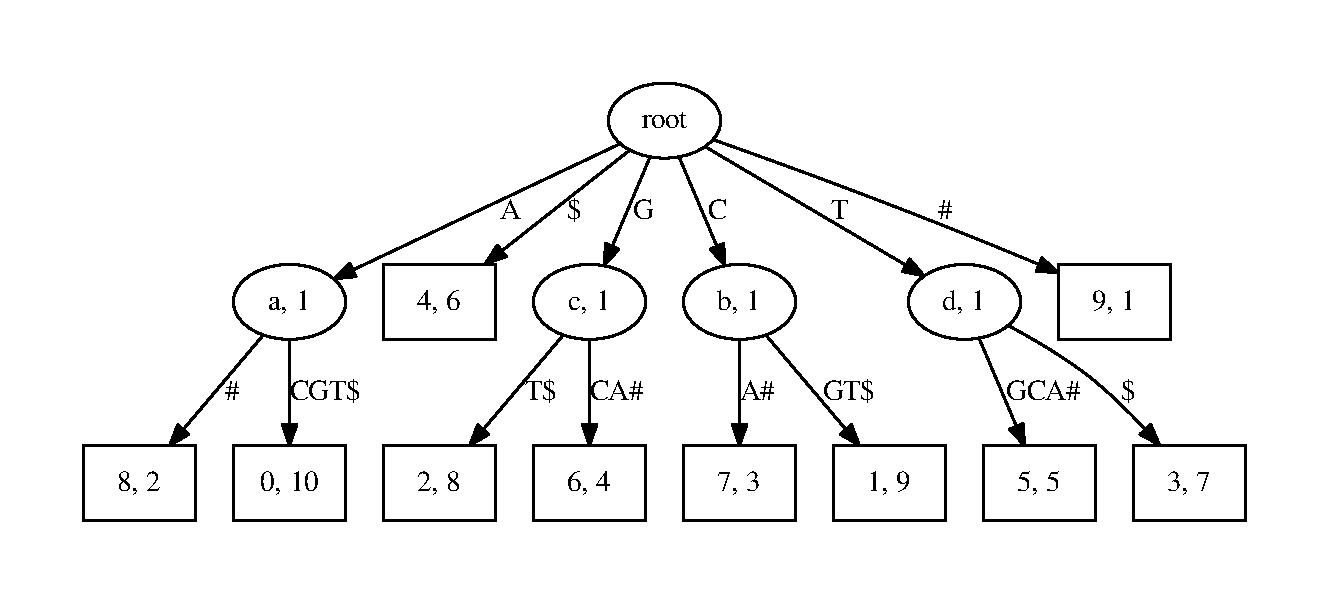
\includegraphics[width=\linewidth]{./img/q1.pdf}
    \caption{Generalized suffix tree.}
    \label{fig:q1}
\end{figure}

\section{Consider a reference genome $T[1..n]$ and a read $R[1..m]$ where $n > m$. We
want to report all positions $i$ such that $Hamming(R, T[i..i+m-1]) \leq k$. Please
propose an $O(kn)$ - time algorithm. (Hint: We can build the suffix tree for
$T\#R\$$ and the corresponding longest common prefix data structure using 
$O(n+m)$ time.)}

\large{\textbf{Answer:}}

This is not easy, and I'm not have enough time, so I referenced some papers. 
In 1989 Landau and Vishkin proposed an approximate string matching algorithm\cite{landau1989fast}.
This algorithm can solve approximate matching problem in $O(kn)$ time.
In the original paper they denote $k$ as edit distance, but here the $k$ as Hamming distance,
so it need to be modified for solve this problem. \\

\pagebreak

\noindent
\textbf{Algorithm description:} \\

We use $V(i,j)$ denote the Hamming distance between the $R[1..i]$ and $T[j-i..j]$.
For example, when $T=GGGTCTA$ and $R=GTTC$, $V$ will be look like this:

\begin{center}
\begin{tabular}{|c|c|c|c|c|c|c|c|}
    \hline
      & G & G & G & T & C & T & A \\
    \hline
    G & 0 & 0 & 0 & 1 & 0 & 1 & 1 \\
    \hline
    T &   & 1 & 1 & 0 & 2 & 1 & 2 \\
    \hline
    T &   &   & 2 & 1 & 1 & 2 & 2 \\
    \hline
    C &   &   &   & 3 & 1 & 2 & 3 \\
    \hline
\end{tabular}
\end{center}

Then we use $L_{d,e}$ denote the largest row in the $V_{d}$, that satisfy $V(row, row+d-1) \leq e$.
Where $V_{d}$ is the $d$-$th$ diagonal in the table $V$. For example $V_1=0,1,2,3$ $V_2=0,1,1,1$ ...
Clearly, if $L_{d,e} = m$ and $e \leq k$, we can say that $Hamming(R, T[d..d+m]) \leq k$. 
So our goal is equivalente to find all $d$, that $L_{d,e}=m$ where $e \leq k$.

Actually, according to Landau and Vishkin's proof\cite{landau1989fast}, $L_{d,e}$ can be computed by a dynamic programming 
algorithm. 

\begin{algorithm}[H]
    \SetKwInOut{Input}{input}\SetKwInOut{Output}{output}
    \SetKwFunction{print}{print}
    \SetKwFunction{initialize}{initialize}

    \Input{$T[1..n]$, $R[1..m]$, $k$}

    \initialize{$L_{d,e}$, $T$, $R$}

    \For{$e \leftarrow 1$ \KwTo $k$} {
        \For{$d \leftarrow 1$ \KwTo $n-m+1$} {
            $row \leftarrow \max{\{(L_{d,e-1}-1), (L_{d-1,e-1}), (L_{d+1,e-1}+1)\}}$ \\
            \While{$(row < m) \wedge (row+d < n) \wedge (R[row+1]=T[row+d+1])$} {
                $row \leftarrow row + 1$
            }
            $L_{d,e} \leftarrow row$ \\
            \If{$L_{d,e} = m$} {
                \print{d}
            }
        }
    }
    \caption{Dynamic programming for compute $L_{d,e}$}
\end{algorithm}

Then we discuss the base case of this dynamic programming algorithm:

Firstly we build the generalized suffix tree of $T$ and $R$.
The base case $L_{d,0}$ equal to find the LCP(Longest Common Prefix) of $R$ and $T[d..d+m]$.
This can be done in $O(1)$ time.

\begin{algorithm}[H]
    \SetKwFunction{initialize}{initialize}
    \SetKwProg{Fn}{procedure}{}{end}

    \Fn{\initialize{$L_{d,e}$, $T$, $R$}} {
        $L_{0, e} \leftarrow 0$ \\
        build generalized suffix tree $\tau$ of $T$ and $R$ \\
        \For{$d \leftarrow 1$ \KwTo $n-m+1$} {
            $L_{d,0} \leftarrow LCP(R, T[d..d+m])$
        }
    }

    \caption{Base case initialization}
\end{algorithm}

\ \\

\noindent
\textbf{Time analyze:}

In this algorithm, build suffix tree take $O(m+n)$ time.
For table initialization, need fill $n-m+1$ entry, each entry take $O(1)$ time,
so this step take $O(n)$ time. 
Fill the full table $L_{d,e}$ take $O(kn)$ time.
So whole algorithm can be done in $O(kn)$ time.

\section{Consider $S_1$=$AAAACGTCGGGATCG$ and $S_2$=$GGGCGTAAAGCTCT$.
Suppose the minimum length of MUM is 3. \\
(a) What is the set of MUMs? \\
(b) If we further require that the MUMs are also unique in the sequence
and its reverse complement, what is the set of MUMs?
}

\large{\textbf{Answer:}}

(a): The set of MUMs is $\{CGT, GGG\}$

(b): If consider unique in the reverse complement sequence, the set of MUMs is:
$\{GGG, CCC\}$

\section{Let $A$=$1 2 3 ... 9$ and $B$=$9 6 1 4 7 2 3 5 8$. Suppose we run the $O(n log(n))$ -
time algorithm to find the longest common subsequence. Can you report the
list of tuples stored in $T_i$ for $i$=$0, 1, ..., 9$? Please discuss how do you construct
$T_i$ from $T_{i-1}$.
}

\large{\textbf{Answer:}} \\

\begin{tabular}{l|l}
    \hline
    i & $T_i$ \\
    \hline
    1 & \{(2, 1)\}\\
    2 & \{(2, 1), (5, 2)\}\\
    3 & \{(2, 1), (5, 2), (6, 3)\}\\
    4 & \{(2, 1), (3, 2), (6, 3)\}\\
    5 & \{(2, 1), (3, 2), (6, 3), (7, 4)\}\\
    6 & \{(1, 1), (3, 2), (6, 3), (7, 4)\}\\
    7 & \{(1, 1), (3, 2), (4, 3), (7, 4)\}\\
    8 & \{(1, 1), (3, 2), (4, 3), (7, 4), (8, 5)\} \\
    9 & \{(0, 1), (3, 2), (4, 3), (7, 4), (8, 5)\}
\end{tabular} \\

Construct $T_i$ from $T_{i-1}$:
\begin{enumerate}
    \item Delete all tuples ($j$, $C_{i-1}[j]$) where $j \geq \delta(i)$ and $C_{i-1} \leq C{i-1}[\delta(i) - 1] + 1$
    \item Insert $(\delta(i), C_{i-1}[\delta(i)-1]+1)$
\end{enumerate}

My implementation see: \\
\url{https://github.com/Nanguage/Course-Algorithms-in-Bioinformatics/blob/master/L09/bs_lcs.py}.

\bibliographystyle{unsrt}
\bibliography{ass3}

\end{document}